\documentclass[12pt]{article}
\usepackage{graphicx}
\usepackage[section]{placeins}
\usepackage{amsmath}
\usepackage{enumitem}
\usepackage{tcolorbox}
\usepackage{subfigure}
\usepackage{amssymb}
\usepackage{hyperref}

\title{Controlled Procedural Terrain Generation}
\author{Alfredo Russo}
\date{A.A. 2021-2022}

\begin{document}
    \maketitle
    \newpage
    \tableofcontents
    \newpage
    

    \section{Introduction}

    \section{Coastline Agent}

    \section{Smoothing Agent}
    Smoothing agent is the one which deals with smoothing points previously elevated by the coastline agent.
    In order to do that it use extended Von Neumann neighbourhood, changing the height of the points.
    The agent perform a random walk on the map changing those heights.
    
    \subsection{Agent parameter}
    Like every agent it has parameters that allow designer to led different results based on it.
    These parameters are:
    \begin{itemize}
        \item \textbf{AgentNr:} it represents the number of agent that will be placed on the map in order to smooth coastline points.
        \item \textbf{returnValue:} this is a value used for understand when the agent have to came back to its starting point. The more the value is high, the more
        the points near the starting point will be smooth. So the agent came back to the starting point periodically and this is useful if some parts of the map need 
        more smoothing than others.
        \item \textbf{smoothingTokens:} it represents, like all other agent, the number of action that the agent can perform. The more the number is high, the more the map will be smooth.
    \end{itemize}

    For speeding up the computation there is another parameters taken by the coastline script which is \textbf{coastline points}, so the points where it is possible to place the agent.
    This is done because retrieving coastline points (points which height is more than 0) can be perforamce expensive depending on how much the map is big. 

    \noindent 
    Smoothing agent require terrain to work, so there are all the parameters related to the terrain like \textbf{terrain data}, \textbf{heightmap} and so on \dots

    \noindent
    There is also a parameter called \textbf{neighboringPoint} which is used when the agent have to move itself in an adjacent point.
    
    \noindent
    At the end there is an instance of the smoothing agent in order to let the agent start working after and only after the coastline agent finish its work.

    \subsection{Action}
    This method represents the agent action on the map, but before it can start smothing points there are a couple of thing to do.
    The first thing is to retrieve all the heights related to map points previously generated by the coastline agent. So the heighmap matrix is filled with this information.
    The second one is to retrieve all the coastline point (the point with heights greater than 0) in order to place the agents on the map. This is done by retrieving the
    related hashset by the coastline agent script in order to avoid useless computation. Furthermore the complexity of this kind of computation increase with the map size 
    because it is nedeed to check every point height of the map.
    After these things the action can start.

    Every agent need to be placed on the map but not in a completely random way. The agents have to be placed on a coastline point, so in order to do that a random point is retrieve
    from the haseset which contains them and assigned to the starting point. This point is very important for the smoothing agent because, as previously said, this agent returns
    to its starting point periodically.

    In order to understand when the agent have to return to its starting point it is used a counter (\textbf{count}) originally set to 0;
    
    It is important to track the position of every agent and for this is used a variable called \textbf{location} that it is updated during time with the current agent postion. 
    At the beggining it is set to the value of the starting point.

    Every agent can perform an action according with the number of the tokens specified. The action can consist of came back to the starting point or change the height of a point
    with extended VonNeumannNeighborood.

    If the value specified as \textbf{returnValue} is 5, it means that the agent have to came back to the starting point 5 times. In order to compute after how many action the agent
    have to came back, the number of tokens is divided by the returnValue. So if the counter is greater than this value the agent have to came back, the location is set to the
    starting point and the counter is set to 0. Otherwise the agent can perform its action computing the new height for the point where it is and then update the value in the haightmap.
    After this, the agent move itself on a valid random neighboring point thanks to the \textbf{GetNeighboringPoint} method and the counter is incresed by one.

    I choose to use unity coroutine, so every time an agent end its work, the terrain is updated with the new heighmap values.

    \subsection{VonNeumannNeighborood}
    The VonNeumannNeighborood method compute the new height of the given point p as the average of points in an extended von Neumann neighborhood of p consisting of the
    four orthogonal map points surrounding p on the elevation grid and the four points beyond these, see \ref{fig:vonNeumann}.
    \begin{figure}
        \centering
        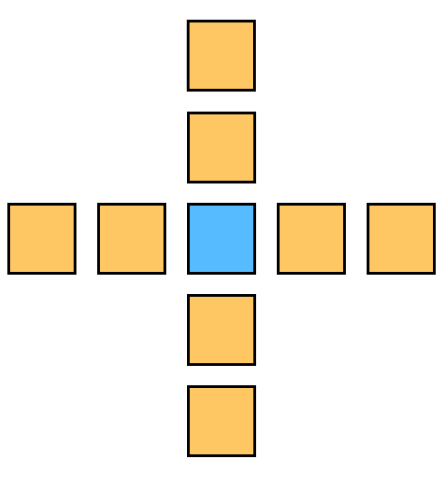
\includegraphics[scale = 0.7]{images/Extended VonNeumannNeighborhood.png}
        \caption{Extended Von Neumann Neighborood}
        \label{fig:vonNeumann}
    \end{figure}

    \noindent
    A weighted average height is calculated, with the center point given 3 times the weight of the other points. Therefore nine points with a total weight of eleven are used.
    Starting from this information it is possible to calculate the weight for the central point and the weight for the surrounding points resolving the following equation system:
    \begin{equation}
        \begin{cases}
            x + y = 11
            \\ 3x = y
        \end{cases}
    \end{equation}

    \noindent
    The variable x represents the weight for the central point which is 3 times the other points weight represented by y. So the central point weight is 11/4 and other points weight is 33/4.

    Then the heights of all the points are collected, but it can happen that a surrounding point of location is outside the map. In this case as height is considered the one of the location
    itself. This choice is done because if it is considered as height for the points otuside the map the value 0, what happens is that the coastline near the end of the map will be smoothed 
    until the height of the points near the end of the map is 0.
    
    After collected all heights the weighted average height is calculated as follow:
    \begin{equation}
        a = \dfrac{\sum\limits_{i=0}^{9} (W_i * H_i) }{\sum\limits_{i=0}^{9} W_i }
    \end{equation}

    \noindent
    Where W represent the weight and H represent the height value. 

    \subsection{GetNeighboringPoint}
    This method takes the current location of the agent and starting from this check if the neighboring point are inside the terrain and then add it to a list. After it is choosen a 
    random point between the valid one found.

    In order to check if a point is inside the terrain it is used the method called \textbf{IsInsideTerrain} that check if the coordinate of the point are between the range 0 and
    the limit of the map.

    \section{Beach Agent}

    \section{City Agent}

    \section{Tree Agent}

    \section{Harbor Agent}

\end{document}